\section{440 --- K-th Smallest in Lexicographical Order}
Given integers $n$ and $k$, find the lexicographically $k$-th smallest integer in the range from 1 to $n$.

\paragraph{Note:} 
\begin{itemize}
\item $1 \leq k \leq n \leq 109$.
\end{itemize}

\paragraph{Example:}

\begin{flushleft}
\textbf{Input}: $n=13$, $k=2$

\textbf{Output}:10

\textbf{Explanation}: The lexicographical order is $[1, 10, 11, 12, 13, 2, 3, 4, 5, 6, 7, 8, 9]$, so the second smallest number is 10.
\end{flushleft}

\subsection{十叉树}
数字的字典序可以用如下的十叉树来表示
\begin{figure}[H]
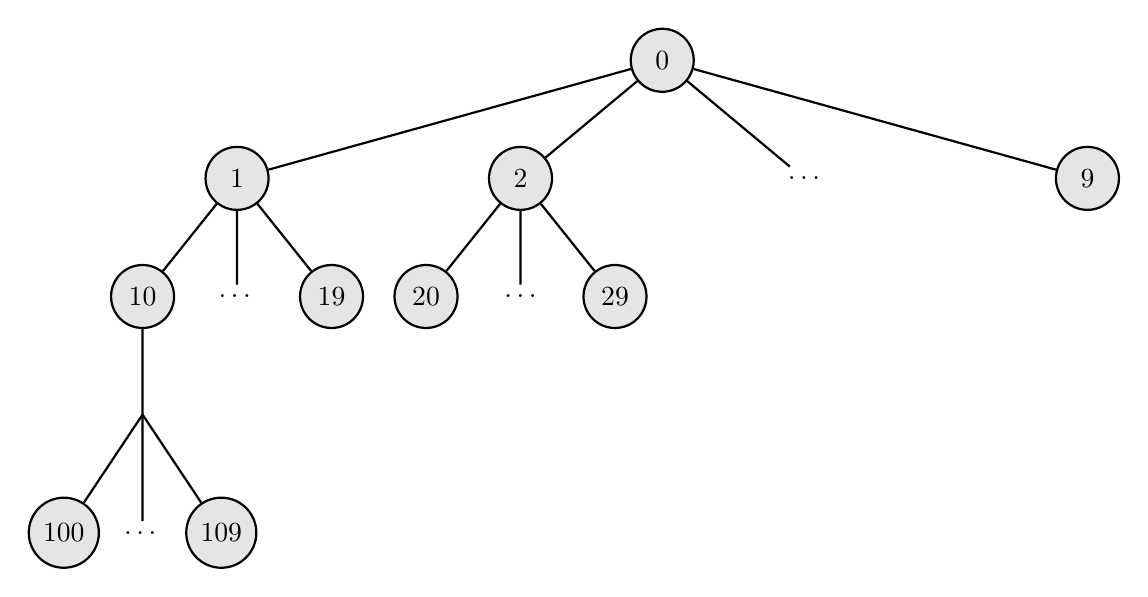
\begin{tikzpicture}
[my/.style={draw, minimum size=8mm, circle, fill=gray!20!}, thick,
level 1/.style={sibling distance=36mm}, level 2/.style={sibling distance= 12mm}, level 3/.style={sibling distance=10mm}]
\node[my](0) at (0,0) {0} 
child{
node[my] {1} 
child{
node[my] {10}
child{
	child {node[my] {100}}
	child {node {\ldots}}
	child {node[my] {109}}	
}
}
child{node {\ldots}}
child{node[my] {19}}
}
child{
node[my] {2}
child {node[my] {20}}
child {node {$\ldots$}}
child {node[my] {29}}
}
child{node(3) {$\ldots$}}
child{node[my](4) {9}};
\end{tikzpicture}
\end{figure}
preorder traverse这个tree就可以得到字典序。但是如果$k$很大,按照preorder traverse一个个的遍历显然是不可取的,需要找到快速jump的方法。
\begin{itemize}
\item 首先计算出从当前number $x$到$x+1$需要多少steps。
\item 如果total steps小于$k$,则表明$x$能跳到$x+1$。否则,则按照preorder遍历的方式前进一个step,而$x$跳到$x\times 10$。
\item 计算$x$和$y$之间的steps的方法: 
\begin{enumerate}
\item $x$和$y$之间的steps由$n$来决定,因为$n$决定了十叉树的深度。
\item 按照$x$和$y$在同层之间的间距来得到steps,例如$1$到$2$,在第一层,1到2的steps就是1。然后同时跳到第二层,这时候1变为10, 2变为20,10到20的steps就是10。
\item 做循环直到$x > n$,在每次循环中,计算$x$和$\min(n+1, y)$之间的差值加入到总的steps中。然后$x$和$y$同时跳到下一层,即$x\gets x\times 10$,$y\gets y\times 10$。
\item 
之所以选择$n+1$是因为$n<y$时,需要jump到$n$上。例如从$x=1$到$y=2$,$n=10$,当$x$和$y$都前进到下一层分别变为10和20,如果选择$\min(n,y)$,那么$\min(n,y)-x$就为零,但是我们需要从1跳到10这一个step。所以正确选择是$\min(n+1,y)$。
\end{enumerate}
\end{itemize}

\setcounter{lstlisting}{0}
\begin{lstlisting}[style=customc, caption={Prorder Traveseing With Jump To Tenary Tree}]
int findKthNumber( int n, int k )
{
    int total = 1;
    int x = 1;

    while( total < k )
    {
        int steps = cal_steps( n, x, x + 1 );

        if( total + steps <= k )
        {
            //since total are no larger than k
            //x can jump to x+1
            total += steps;
            x = x + 1;
        }
        else
        {
            //otherwise, jump down with one step
            //to next level by preorder traversing
            //x jump to x * 10
            ++total;
            x *= 10;
        }
    }
    return x;
}

//get steps between  x and y, and maximum number is n
int cal_steps( int n, int x, int y )
{
    long long steps = 0;

    //change to long long to avoid
    //overflow
    auto ln = static_cast<long long>( n );
    auto lx = static_cast<long long>( x );
    auto ly = static_cast<long long>( y );

    while( lx <= ln )
    {
        //notice: we need ln+1 not ln
        //to count for the step from x=n to n
        steps += ( min )( ln + 1, ly ) - lx;
        lx *= 10;
        ly *= 10;
    }

    return steps;
}
\end{lstlisting}